\section{Background}
\label{s:background}

\begin{figure*}[t]
\centering
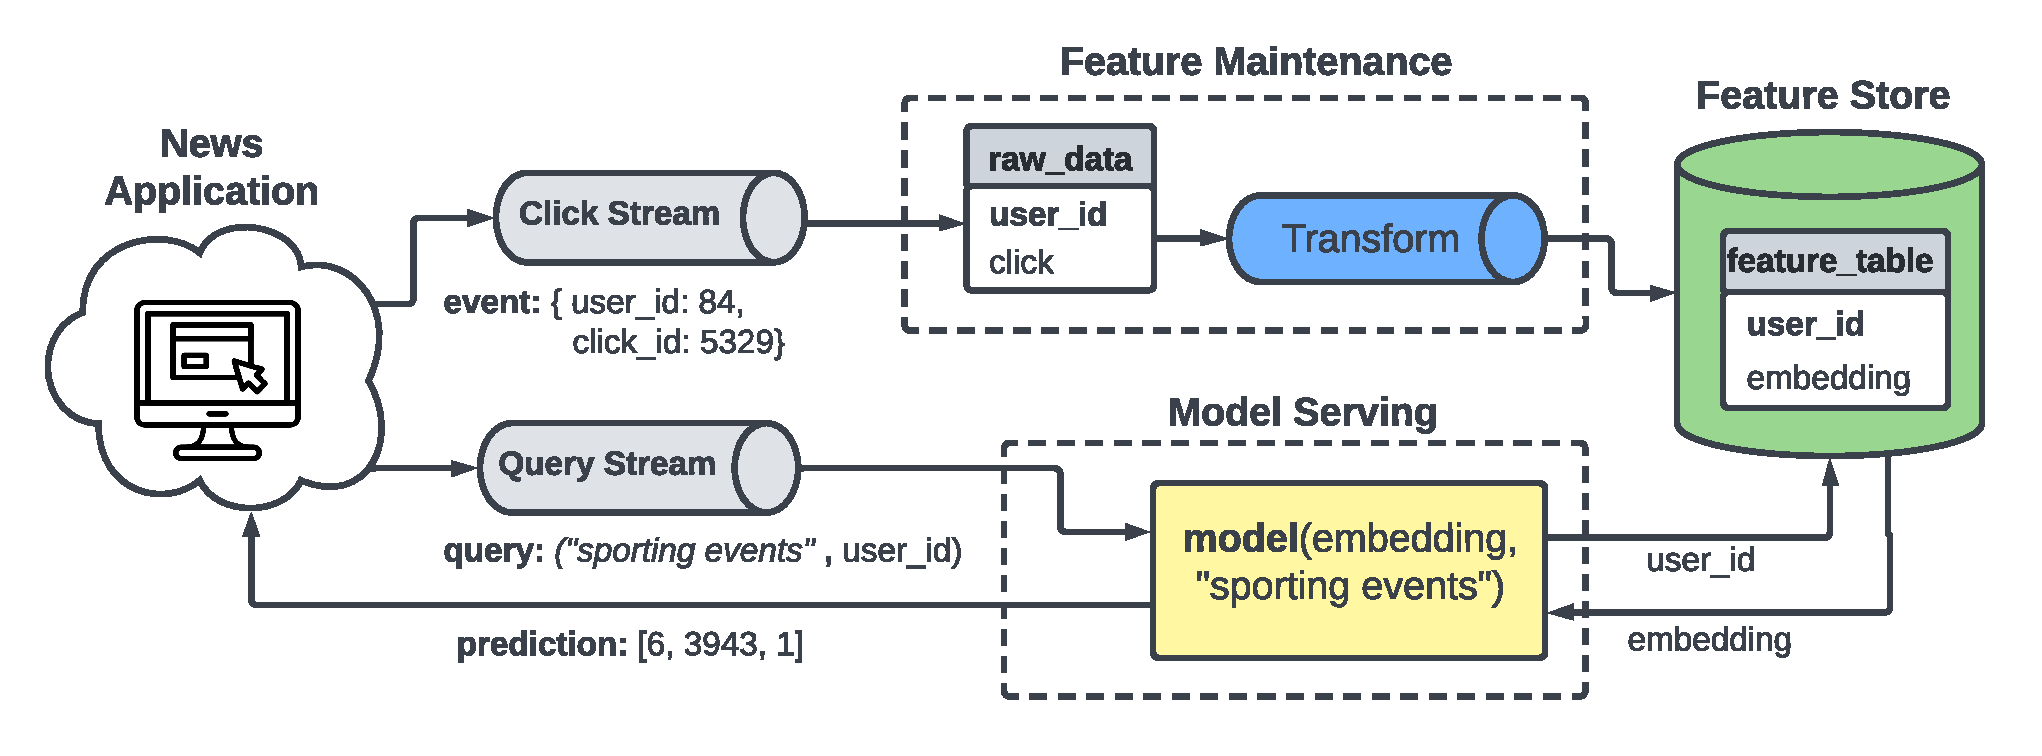
\includegraphics[width=14cm]{ralf/figures/feature_store.pdf}
%\setlength{\belowcaptionskip}{-10pt}
%\setlength{\abovecaptionskip}{10pt}
\caption{A ML serving pipeline with a feature store. 
%for a news application logging user clicks (\textit{click/event stream}) and submitting queries to a model when the user makes search requests (\textit{query stream}). 
%The model looks up the user's embedding, derived from historical click data, as an additional input to make a prediction (e.g. a list of recommended article IDs). 
}
\label{f:feature-store}
\end{figure*}

Most machine learning applications rely on \emph{features} to summarize relevant aspects of the training data and provide the necessary context to make informed predictions.
To illustrate, we return to our 
online news recommendation service example (\S\ref{s:introduction}). 

In this setup, the model $m$ must predict the probability $\hat{y}$ that user $u$ will click on article $a$ given a search query $x$.  
Most papers in the area will denote this seemingly simple prediction task as
\begin{equation}
    \hat{y} = m(x, u, a).
\end{equation}
 \amit{Papers in the machine learning and systems community often advance methods to design, train, and efficiently compute the model $m$. In this paper, however, we focus on how to compute the features $u$ and $a$ to optimize accuracy.} \joey{I don't know if we need this change here did the reviews not like the informality of the writing.} \amit{R3 said "Also, the authors should tone down this overstatement: ”After all, most papers in the machine learning and systems community are about how to design, train, and efficiently compute the model m.”"}
 After all, most papers in the machine learning and systems community are about how to design, train, and efficiently compute the model $m$. 
In this paper, we focus on how to compute the features, $u$ and $a$, to optimize accuracy. 

Hidden in this notation is the need to transform \textit{historical data} associated with the user $u$ and article $a$ into their respective features, which can encode everything from the user's entire click history, to the contents of the article, and even the histories of other users that clicked on that article.
As a consequence, a more accurate notation for this task would be:
\begin{equation}
    \hat{y} = m\left(x,
    f_\text{users}\left(\mathcal{D}^{t}_u\right), 
    f_\text{articles}\left(\mathcal{D}^{t}_a\right) 
    \right), 
\end{equation}
where the functions $f_\text{users}$ and $f_\text{articles}$ are \emph{featurization functions} and $\mathcal{D}^{t}_u$ and $\mathcal{D}^{t}_a$ are all the data up until the present ($t$) that is associated with the user and article.
Each of the feature functions returns a vector that is combined with the query text $x$ and processed by the model $m$. $m$ makes a prediction, calculating the probability that user $u$ will click the article $a$.

While the aforementioned example described only a couple of features, in practice, there may be dozens of features from different data sources computed for a single prediction. Automated feature generation tools make is easy to generate hundreds of unique features from data \cite{feature-tools}. For notational simplicity, in this paper we will focus on a single featurization function $f$ and key $k$:
\begin{equation}
    \hat{y} = m\left(x, 
    f\left(\mathcal{D}^{t}_k\right)
    \right). 
\end{equation}
where $x$ is the query and $\mathcal{D}^{t}_k$ is the historical data for key $k$. 
%\natacha{Should we make it explicitly clear here that we are therefore assuming that the features are independent from each other? I don't think we have explicitly stated this assumption anywhere}
% However, the techniques we introduce apply to settings with additional feature functions. 
% \joey{maybe drop the last sentence.} \natacha{grammar}\joey{yep.}

Querying available historical data $\mathcal{D}^{t}_k$ and computing the featurization function $f$ for each prediction request may be prohibitive in low-latency prediction serving settings where recommendations must be generated in real-time a users are scrolling through their news feed.
% \natacha{note, this suggestst that there's two issues, the large data size, and the cost of th function. is that true?} \joey{yes, we probably should actually address each part separately and in this paper we sort of side step the access costs and focus on computation.  Possibly a mistake.}
Each query may need to access large amounts of historical data and run a computationally expensive feature function $f$. For example, many recent content recommendation models employ deep learning techniques to encode click streams and article contents and run online gradient descent~\cite{DLRM19}.
%

Furthermore, many predictions may query the same keys, resulting in redundant computation. Often the same user features will be used to rank multiple articles and the same article will be ranked for many users. Executing the query on the entire history of users and articles for each new prediction is redundant, expensive, and infeasible for latency constrained settings.

% For the prediction serving application to generate features for some key $k$ when a prediction query is made, the application needs to lookup the current $\mathcal{D}^{t}_k$ available for key $k$ from some data table, \texttt{historical\_data}. We can represent the SQL query the prediction serving application makes for features as: 
% \begin{lstlisting}[
%           language=SQL,
%           basicstyle=\ttfamily,
%           numberstyle=\tiny,
%           commentstyle=\color{gray}, 
%           label={lst:select}
%         ]
%     SELECT key, f(data) 
%     FROM historical_data WHERE key=k
% \end{lstlisting}
% where $f$ is the feature function implemented as a UDF. However, the latency of this query may be prohibitive in low-latency prediction serving settings where recommendations must be generated in real-time as as users are scrolling through their news feed. 



To guarantee low-latency feature queries and avoid redundant computation, features are often \textit{pre-computed} and stored in low-latency data store, referred to as \textit{feature stores}. 
% in industry ML pipelines. 




\subsection{Feature Stores}
The \emph{feature store} is a nascent class of systems which target the problem of storing and maintaining feature tables. We show an overview of a how feature stores, model serving, and applications interact in \cref{f:feature-store}. There are several major open-source and commercial feature store systems \cite{featurestoresorg,tecton, hopsworks, amazon}. Feature stores can be used to fulfill a variety of requirements, such as enabling sharing of features across different multiple downstream applications, improving latency and cost by pre-computing features, and managing metadata about features (e.g. version control), which we discuss further in Section ~\ref{s:discussion}. In this paper, we focus specifically on maintaining feature table over streaming data updates in the context of online prediction serving. 

% To eliminate the need to run expensive feature computation when serving low-latency predictions, it is common practice to pre-materialize features and store the values in a \emph{feature table} that is stored in a low-latency data store.  
% The feature table is essentially a materialized view over raw, historical data. Pre-computing feature table values eliminates redundant computation across multiple predictions, and helps meet prediction latency constraints.  feature values can be reused across multiple predictions. 
% \begin{lstlisting}[
%           language=SQL,
%           basicstyle=\ttfamily,
%           numberstyle=\tiny,
%           commentstyle=\color{gray}
%         ]
% CREATE MATERIALIZED VIEW feature_table 
% AS (
%     SELECT key, f(data)
%     FROM historical_data
%     GROUP BY key
% )
% \end{lstlisting}
% \natacha{This might not be the right place yet, but we've not discussed at all the consistency requirements}
%\subsubsection{Feature Maintenance}

% The feature table can be fully refreshed when enough new data is recieved, or we can also update a specific key $k$ with inserts like the following:
% \begin{lstlisting}[
%           language=SQL,
%           basicstyle=\ttfamily,
%           numberstyle=\tiny,
%           commentstyle=\color{gray},
%           escapechar={|}
%         ]
% INSERT INTO feature_table(key, value) VALUES
% (
%     SELECT key, f(data)
%     FROM historical_data
%     WHERE key = |\color{red}{k}|
% )
% \end{lstlisting}

As the underlying, raw data is updated over time, pre-computed features need to be \textit{maintained} to prevent feature staleness, which may degrade prediction quality of dependent downstream models. For example, a feature encoding a user's interests in news topics can change rapidly with each new action by that users. If the feature is not updated over time, the stale encoding may degrade the quality of recommendations made by a model for that user. 

Existing feature store typically rely on external data processing systems (e.g. Spark, Flink) to compute feature updates from new data. These systems then process new data in either a streaming or batch fashion to update current feature values.


\subsection{Feature Maintenance}
Maintaining features with new data can be computationally expensive, depending on the rate of new data arrival, the cost of the featurization function, and the required feature freshness.  While some feature functions can be incrementally applied to new data, many require significant re-computation over a large window of historical data with the arrival of each new record.   
For example, an attention-based text document embedding model will need to re-compute the embedding of the entire document to reflect a single word change. \jmh{give a canonical citation}
\joey{Kevin, maybe we can reference the colBERT paper here?}
Even when feature functions can be applied incrementally, running them in a streaming fashion on high velocity data streams can require expensive computational resources (e.g., GPUs) and be less efficient than large batch updates~\cite{clipper, crankshaw2020inferline}. 


Updating features with every data change can be expensive and unnecessary, depending on how quickly the true feature value is changing and how much impact staleness has on model predictions. In cases where models are robust to stale features, running a daily batch job to process new data is sufficient. In other cases where models are sensitive to feature staleness, features may need to be continuously updated with new data. For example, Splunk uses Flink for streaming maintenance of time-series features for real-time anomaly detection \cite{mishra2021onlinestl}, and has developed application-specific solutions for maintaining fresh features for high cardinality data streams \cite{mishra2021onlinestl}. 
Feature values are typically \textit{eventually consistent} with respect to the underlying raw data.
% \sarah{is this a correct use of the term "eventually consistent"?} \joey{Yeah close enough.}



To provide a specific example, we implement a workload similar to Splunk's in Flink where we maintain a time-series decomposition for a set of cloud virtual machines, each streaming CPU utilization data. Updating a feature for a given virtual machine (i.e. the key) takes about 0.3 seconds, so a single Flink process can only update about 3-4 features per second. Existing systems do not natively have application awareness to prioritize updates, so will use a FIFO queue to process new data in incoming order. As a result, increasing the cardinality of the dataset eventually results in the per-key staleness linearly increasing with time as updates 
lag
% fall further and further behind 
new data, as shown in \cref{f:flink}. These increases in feature staleness are correlated to decreased prediction accuracy, as shown in \cref{f:staleness}.

% %Real-time maintenace can be paticularly challenging when there is a high-rate of incoming data (e.g. high-density clickstreams) and high cardinality (e.g. features for millions of users), requiring a large number of updates to process to maintain fresh features. 
% The increasing importance of maintaining fresh features in the face of these challenges has motivated a number of workload-specific solutions. Tecton has released a blog post citing cost as a barrier to high feature freshness \cite{tectonfreshness} and developed new methods for computing real-time aggregation windows more efficiently \cite{tectontile}. \kevin{This seems a bit outdated to me and I think we can remove it} Splunk faced challenges with featurizing high cardinality data streams with time-series decomposition for downstream anomaly detection models  \cite{mishra2021onlinestl}, motivating development of an online time-series decomposition algorithm. 

In this paper, we show that scheduling feature updates according to each key's impact on downstream accuracy allows us to preserve overall accuracy at lower cost. Feature stores %are uniquely situated between updates to features and feature queried, but 
typically lack awareness of downstream query patterns and performance of the predictions made using queried features. As a result, systems for maintaining features treat all data updates and keys symmetrically and fail to leverage important information about which updates are critical and which keys are likely to be accessed in the downstream prediction workload. 



%Many real-time applications such as recommendation or anomaly detection systems benefit from features which provide \textit{real-time context}. These features are derived by transforming real-time data streams, such as user clickstreams. 

%While more machine learning pipelines move towards leveraging real-time data \cite{chip}, these pipelines struggle to support to support complex streaming transformations (e.g. model predictions) while also maintaining high freshness, especially for high cardinalities. Many recent ML models (e.g. sequence/text models) have high CPU inference latency \cite{huggingface}. Furthermore, high cardinality feature tables (e.g. features for millions of users) may need to simultaneously process updates to many keys concurrently, even if the individual update rate for each key is small. 

% https://blog.roblox.com/2020/05/scaled-bert-serve-1-billion-daily-requests-cpus/
% https://arxiv.org/abs/2102.06621
% https://huggingface.co/blog/bert-cpu-scaling-part-1#4-out-of-the-box-results




\sarah{(TODO: R5. Add a discussion on real world scenarios in which one cannot update all features in time.}
\joey{I think what is here is not bad. I spent some time looking for papers that describe slow feature computation but its hard to find since feature cost is not typically a focus of ML.}

% \textcolor{red}{
% \subsection{Sustaining Expensive Features}
% }
% \textcolor{red}{In cases where the incoming data rate exceeds the throughput of the data processing, the written features will become stale as the data processing engine falls behind. We implement in Flink one of our evaluation workloads (described in SECTION) for maintaining time-series information per cloud VM CPU logs.   Existing systems do not natively have application awareness to prioritize updates, so will use a FIFO queue to process new data in incoming order. We show in \cref{f:flink} how this results in increasingly staleness as the cardinality of the incoming data stream increases. These increases in feature staleness are correlated to decreased prediction accuracy, as shown in \cref{f:staleness}}.

\begin{figure}[t]
\centering
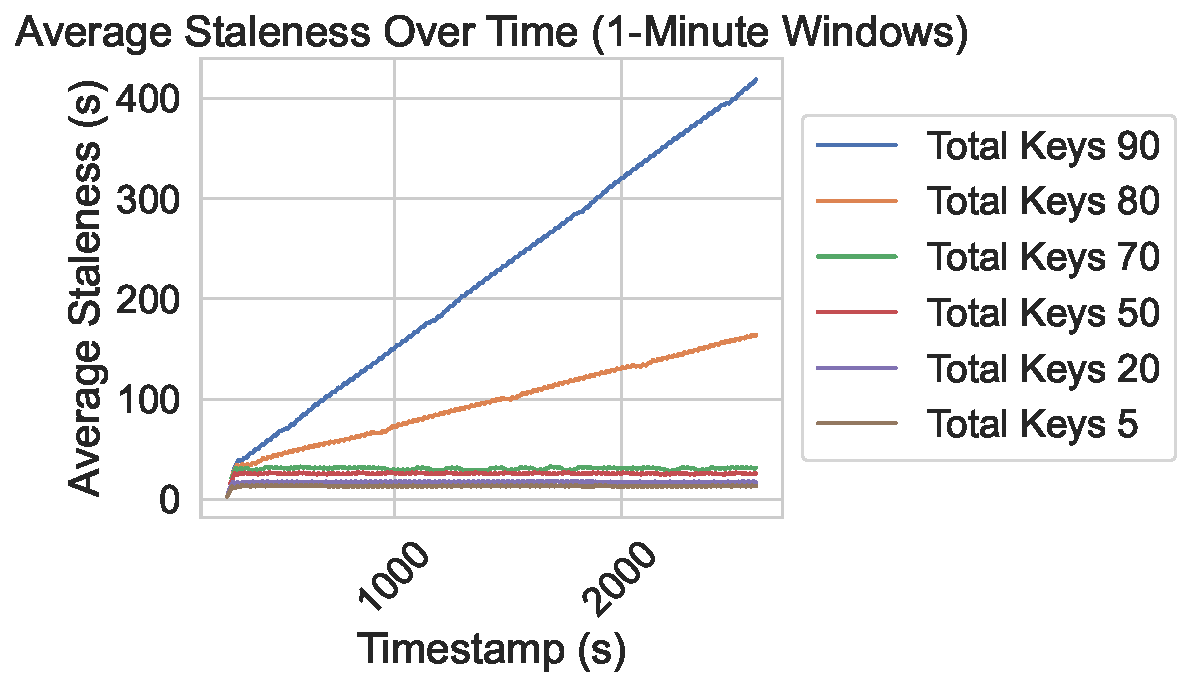
\includegraphics[width=7cm]{ralf/figures/flink.pdf}
\caption{Average staleness in a 1-minute time window across all keys as a function as the cardinality.}
\label{f:flink}
\end{figure}


\sarah{The full Azure dataset has 2 million keys producing data once every 5 minutes, which on lambda  (\$1.7xe-5 per GB-second) would cost \$5,175/day without including data query time. Even supporting 6k active users each producing 10 events/minute costs \$1440/day. Reducing the rate of re-computation naively results in accuracy degradation as shown in Fig 8, 11, and 13.} \amit{We can even specify that this is still a really small use case -- most companies doing some kind of featurization will at least have ~hundreds of features per user, so with a 1M MAU and features calculated every hour on average, it would be cost prohibitive to update.}


%\subsubsection{Consistency Requirements} 
%\textcolor{red}{Reference weak consistency literature from Natacha.} Consistency requirements for feature tables vary across applications and types of features.
%How quickly feature values change over time, and how much they impact downstream model training and inference applications, can significantly vary across different types of features. In cases where models are robust to stale features, running a daily batch job to process new data is sufficient to keep feature up-to-date. In other cases where models are sensitive to feature staleness, features may need to be continuously updated with new data. For example, Splunk uses Flink to maintain time-series features used for anomaly detection \cite{mishra2021onlinestl}. Choosing the frequency of feature updates depends on the cost of featurization, the rate of new data arrival, and the sensitivity of models to staleness. 
 
\subsection{A Feature Store Reference Model}
For simplicity, we first describe the standard formulation of a feature store. 
In Section~\ref{s:discussion}, we discuss the full variety of feature stores presently being used, and how our work applies.

We assume that raw historical data is loaded into a data warehouse, capturing the basic entities (users, movies) and actions (users seeing ads, users viewing movies, etc) we use in prediction. We then consider a derived \emph{feature table} that memoizes \emph{featurization functions} over that data. This table can also be stored in the data warehouse, or it can be maintained in an external cache database like Redis or Memcached; our design does not depend on that decision. A SQL query that populates the feature table exhaustively would have a template that looks like this:
\begin{lstlisting}[
           language=SQL,
           basicstyle=\ttfamily,
           numberstyle=\tiny,
           commentstyle=\color{gray}
        ]
    SELECT key, uda(data)
    FROM historical_data
    GROUP BY key
\end{lstlisting}
where \texttt{uda} is a user-defined aggregate function. If the feature store is kept in the warehouse, feature tables can be viewed as traditional materialized views. 
%it could be represented as a materialized view of the full featurization query.
\jmh{I think some of the discussion here is using a naming scheme that got lost in copying. I think I labeled the query above as ``the featurization query'' (without the materialized view aspect), and the alternative below the ``cache maintenance query'').}
\natacha{Temporarily removed Joe's text for consistency}
Materialized views, however, are typically kept consistent with underlying data, and must be recomputed on every new update. Systems that support incremental view maintenance incur similar costs when the supplied feature function cannot be recomputed incrementally. In contrast, \system{} focuses on carefully choosing when and what keys to recompute to minimize resource costs while preserving accuracy:
\begin{lstlisting}[
           language=SQL,
           basicstyle=\ttfamily,
           numberstyle=\tiny,
           commentstyle=\color{gray},
           label=lst:cache-maintenance
        ]
    SELECT key, uda(data)
    FROM historical_data
    WHERE key IN <PolicyQuery>
    GROUP BY key
\end{lstlisting}
%Our focus in this paper is the design and execution of this maintenance query—particularly the design of the inner "policy query" and the schedule for running the outer Cache Maintenance query
The fundamental policy decision addressed in this paper is: \emph{given the above query can only be run on a small subset of all possible keys at a time \amit{due to cost constraints},
which keys do we select to ensure maximum downstream prediction accuracy. }
\natacha{two issues to me here 1) we're not focused on the design of the query, we're focused on when we choose to execute the query. Second, what's the cache maintenance query? first time we mention it. Old version in text please feel free to add back} We focus on making scheduling decisions across keys (rather than between updates pertaining to a single key), as large key cardinality is a common attribute in feature store applications. We use SQL here to illustrate our ideas, but of course this logic could be implemented in a number of scalable data-centric APIs, including Spark, Flink, and so on.
\sarah{Link back to PolicyQuery in later sections}

\natacha{It felt a little strange to introduce SQL out of nowhere given it's not something you really discuss aywhere else in the paper, etc. Could you do without? Formulating it as a materialized view problem makes sense, it was specifically the sudden "here's SQL code" that was strange to me} 
As we discuss in Section~\ref{s:discussion}, there are many options for materializing and storing features. Our simple model here is designed to be sufficient to illustrate the key policy issues at hand; further architectural complexity is discussed in Section~\ref{s:discussion}.